% TODO: Average increase based on iterations, based on strokes, based on..etc.
% Average time increase based on iter..stroke...etc%  the painting curves... Get control function: takes in the start and end pFixoints, generates two other points along the line that are within reason4

% make background white
% run tests in a sane manner with decent straight lines
% percent increase over
%figure out optimal minimum settings

\chapter{Modified Huffman Coding for Lossless Compression and Bandwidth Optimization}
\section{Introduction}
This project is a compression algorithm based on the Huffman code. We maximize the amount of tokens in the tree in exchange for a smaller compressed message. We avoid having to store the entire Huffman tree with the compressed message by storing it separately, giving an identification number to it and prepending all messages compressed using that code with that identification number, so it can be used to decode it later. Instead of constructing a Huffman code for every single file we compress, we construct a number of generalized Huffman codes based on a category of data and assign each an identification number. These codes and identification numbers together become a ``data context''. We implement a program that holds many data contexts and assigns the best one to each input message and observe how much we can compress messages and how quickly the messages can be decoded

\subsection{The Problem}
Cisco estimates that in 2016, over 96,000 petabytes of data were transferred across networks around the world.\cite{cisco} This is up from 72,000 petabytes in 2015 and for an even more extreme comparison, 12 petabytes in 1998. Clearly, internet traffic is increasing at a great pace. As internet traffic increases, consumers are sending more and more web requests from their client devices every day, with more and more devices to send from. This creates a challenge for those who maintain servers that handle these requests. Savings of kilobytes or even just bytes can add up to have a significant impact on total bandwidth usage when requests are being processed en masse. If there were a way to more effectively compress data before sending it to the client, provided it is quick at both compressing and decompressing and is relatively easy to implement, the savings in bandwidth could be huge, thus providing benefit to any implementing networks. We suggest a compression algorithm and implementation that meets these criteria. 

\subsection{Common Transmission Types}
The majority of traffic on the internet is either text, image, video, or audio. This paper will focus on a text implementation due to the ease of representing text on paper. However, it has already been shown that Huffman code techniques can be used to compress images, video, and audio as well.\cite{huffaudio}\cite{huffimage}\cite{huffvideo} The algorithm we present can therefore also be used on these formats.

Recently, the concept of minimizing Javascript of other web languages has become more and more important. If a large company with a website that is accessed a lot is able to minimize their payload, or filesize of their webpage, they could save lots of bandwidth. Our solution can be used to compress code very efficiently, so this is another reason for focusing on text in our implementation and examples.

What is important is that all common network traffic types can be tokenized, and when tokenized, there is at least some redundancy present. This is when minimum redundancy codes such as the Huffman code are most useful and effective. Note that there is a lot of redundancy in Javascript code (and most code) in the form of variable names, bracketing, keywords, etc., making it a great target for Huffman-based compression. Even if there is not that much redundancy, a Huffman code can be used to hold sets of equivalently occurring tokens to save memory.\cite{huffmemeffic} A Huffman code based solution is therefore very adaptable to the terrain of modern data transmission.

\subsection{Proposed Solution}
Bandwidth is clearly the core concern. We could minimize bandwidth with all sorts of lossy compression, but lossy compression is not acceptable in an algorithm designed for all kinds of web traffic and could result in corrupted data. We seek to minimize bandwidth usage with only lossless techniques.

As memory and data storage device prices decrease every year, it is becoming less and less important to be efficient in space complexity.\cite{mccallum} The traditional Huffman code is fairly conservative in its use of space. We seek to take advantage of this modern trend by inflating the size of the compression and decompression programs themselves in exchange for a smaller compressed file size and thus better compression ratio. Transmitting this smaller file will then use less bandwidth.

From a high level perspective, the version of the Huffman code we present has two major deviations from the original specification. The addition of a data context and the offloading of the Huffman code tree itself into the implementation specification, saving the output file from having to store the entire tree. The addition of a data context has been discussed before, but it has not been as large or offloaded as ours is.\cite{huffimage} We also introduce the concept of a compression benefit. That is, the benefit of compressing something big is more than compressing something small. This will be discussed more later.

A Huffman code is constructed by breaking apart an input message into tokens and constructing a tree based on those tokens and how frequently they occur, with the most frequently occurring tokens at the top of the tree. This tree can then be traversed to encode or decode messages. An example of a traversal represented as a binary string is shown in Figure \ref{fig:hufftraversal}. In this example, $0$ represents going to the left child and $1$ represents going to the right child. The tree itself and the traversal are then written to the disk in an efficient manner, providing a compressed file. If the tree grows too large, then writing it to the output file could make the output file larger than the original input. This is why the Huffman code's most common used method of tokenizing an input is by the letters and symbols used in English, ensuring that no more tokens than the English alphabet and some other symbols are encoded. As this sort of memory conservation is not important in our implementation, we want to choose a less granular token. In our example of English text, we could choose a word or small phrase. We will use a word, as implementing a decision algorithm for determining what constitutes a small phrase is not the focus of this paper, but such an algorithm could be a great addition.

With these less granular symbols, in our case words, we can then construct a much larger Huffman code tree based on the text. This tree should not be based on one individual file, rather, a corpus based on some genre of text. These subsets should be similar in genre, providing a more accurate tree. As an example, if one were to construct a Huffman code tree on all papers submitted to a computer science journal and then use that code to compress the next submitted paper, it would probably do a decent job. If that code was then used to compress all tweets made in the past hour, it would probably not compress that file very well, barring some extreme coincidence. This genre-generalized Huffman code tree is the ``data context'', or context of the data being transmitted.

We then take this very large data context, created from a corpus of computer science academic papers, and store it in the encoding/decoding program with an identification number. The identification number is a fixed-length message before the actual encoded message that specifies which data context was used to encode this message. The output file then does not have the large Huffman code tree in it taking up space, rather, it has an identifier for a data context that it will be paired up with when it is received and decoded.

There is also the consideration of benefits. If the word ``a'' occurs extremely frequently in the input, it will be in one of the top levels of the Huffman code and be compressed down to a very small size. However, if we compress the word ``the'' down to that same small size, even if ``the'' is less frequent, we are potentially (depending on the frequency of occurrence of ``the''), going to be compressing more efficiently. For the sake of example, assume a one-byte letter size and the token is on the third level of the tree, meaning a three-bit compressed token size. We would be removing 5 bits from the representation of the token ``a'' and 21 bits from the representation of the token ``the''. The benefit of compressing a symbol is the frequency at which it occurs times the size of that token. We then use these benefit values instead of the normal frequency value used by a standard Huffman code.

As decoding a compressed file using a Huffman code is very fast, this file can be decompressed quickly.\cite{fastdecode} We also considered using different branching factors to minimize the depth of the tree, but this turns out to have no real impact on output file size. %TODO citation here

\begin{figure}
\centering
    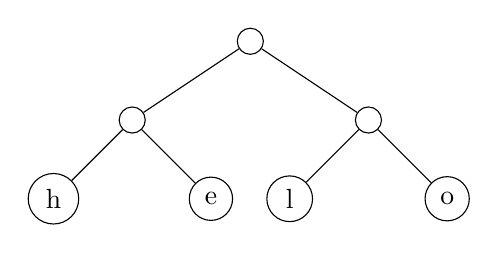
\begin{tikzpicture}
    \node [circle, draw] (e) at (1, 0) {};
    \node [circle, draw] (l) at (2.5, -1) {};
    \node [circle, draw] (h) at (-0.5, -1) {};
    \node [circle, draw] (o) at (-1.5, -2) {h};
    \node [circle, draw] (w) at (0.5, -2) {e};
    \node [circle, draw] (r) at (3.5, -2) {o};
    \node [circle, draw] (d) at (1.5, -2) {l};
    \draw  (e) edge (h);
    \draw  (h) edge (o);
    \draw  (h) edge (w);
    \draw  (e) edge (l);
    \draw  (l) edge (d);
    \draw  (l) edge (r);
    \end{tikzpicture}
    
    0001101011
    
    \caption[Huffman code example]{A rudimentary Huffman code tree with a corresponding binary string that encodes the string ``hello''. A ``0'' in the string corresponds to going to the left child of a node, and a ``1'' corresponds to going to the right. }
    \label{fig:hufftraversal}
\end{figure}


\section{Implementation and Methods}

\subsection{Specification}

The implementation of this algorithm has two parts: a client and a centralized server that keeps track of data contexts. The client needs to have access to a set of standard data contexts (Huffman code trees), their identifiers, and have the ability to traverse them to decode or construct a lookup table to encode a message. The server needs to store all data contexts and their identifiers and provide updates to the clients when needed.

The client as described here is not the typical web definition of a client as a browser, it is an implementation of our algorithm to encode or decode messages. The clients will requests new contexts from the server if they come across a context identifier for which they do not have the context. The client will also be tasked with determining which context, given its current inventory, is most efficient. The simple, and slowest, way to do this is to compress the message with every potential data context and pick the best one. There are much better ways to do this using genre classification, which is an entire field of its own. What is important here is that the process of deciding which context would be optimal does not have to be a brute force solution like what we are using. We used that in our implementation that for simplicity's sake, though. Because the decision of which data context to use must be done when encoding, the process of encoding will indeed be slower than decoding. This is okay, as it could be done in advance (not on the fly as requests are made) to all files being sent. For dynamically generated files, a smarter classification algorithm would be needed to assign an optimal data context on the fly.

%TODO: out of place?
An encoded file consists of the context identifier, the compressed data, and any tokens that were not found in the data context at the end. This is necessary because, as the contexts are not generated based on the input file itself, it is possible for an input file to have tokens in it that are not in the context. There will be a node in the data context that is in the least likely position, a leaf at the farthest level of the tree, that will be a placeholder. The tokens not present in the data context are then stored in their original form at the end of the file, in the same order that the placeholders occurred. This does mean that if a very malicious input message were to somehow circumvent all available contexts and contain a large amount of tokens that no context contained, it would be possible for the message to actually expand instead of being compressed. This is, however, both extremely unlikely and could be checked by comparing the output message size to the input message size and opting not to compress in this case.

The context identifier at the beginning of the file would be however long the implementers feel necessary for it to cover all contexts they would desire. This sort of decision has been historically difficult to make correctly, as the popularity of a particular system is hard to gauge at its inception (e.g. IPv4). In our implementation, it was three bytes, with an option to check the end of the file for more version info if all three bytes were 255. 

\subsection{Advantages}
The solution to the problem of bandwidth optimization is the primary advantage. This algorithm can cut down on file sizes in transmission by immense amounts. This algorithm also can be implemented easily, without much more difficulty than a regular Huffman code. This is important, as the adoption of this algorithm would require browsers to implement decoders and servers to implement encoders (clients and servers here referring to the web sense of the words, not our specification's definition). It is also adaptable to many different data formats and allows for a lot of data contexts, so a data context can fit a specific input message very well.

\subsection{Disadvantages}
Corner cases do exist. It is hypothetically possible for a file to expand, or get abysmal compression. We do avoid this as much as possible, but there will theoretically always be some heinously complicated input that could not be compressed very efficiently. This would not happen in general, though.

The disk space required to store so many data contexts could become very large, especially when accounting for different data types (audio, video, etc.). We assume disk space is not an issue, however, and disregard this.

Lastly, this algorithm is not very good at handling random data or noise. If a person is browsing their computer late at night and drifts off to sleep, their head could hit the keyboard and generate the string ``ugibigbnhdfvbsmdofu''. This would most likely not belong to many contexts, and if it did, that context would not fit the rest of the text very well. This is not too big of a problem, though, as it will just remain uncompressed via the placeholder nodes in the context. The implementer also has the choice to be more smart about these situations and perhaps resort to a different compression algorithm.

\subsection{Our Implementation and Strategy}

Our implementation used the programming language Rust, for its speed and ease of implementing low-level data structures safely (i.e. without memory leaks or things of that nature).

The construction of this tree can be seen in the appendix as Figure \ref{fig:newdatacontext}. First, the corpus is split up on spaces. In a more efficient implementation, punctuation would also be its own token, but I have omitted this from the appendix for brevity. These tokens are then stored as tuples with their benefits, calculated as their length times their size. These tuples are then inserted into a priority queue/min heap strucure which is popped repeatedly to constructed the Huffman code. A lookup table for quicker encoding is constructed from the code for all tokens it contains. Finally, some identifier (arbitrary at this point) is attached to the code to form a data context. 

For encoding, each token is found in the lookup table with its corresponding encoded form. For decoding, the data context traverses the Huffman tree following the traversal prescribed by the binary encoded file. This means that encoding is $O(n)$ where $n$ is the number of tokens in the input and decoding is $O(m)$ where $m$ is the size in bits of the encoded message. Both are very fast operations.

\section{Results}
We constructed a few data contexts that are representative of data frequently transmitted over the internet, namely minified Javascript, English text sourced from novels, and social media English text (a corpus of tweets). We compressed another sampling of texts from the same genre as the data context and averaged the compression ratios to get the values seen in Table \ref{table:compressionResults}.



One particular advantage of using a Huffman coding in this manner is the bit-level output of the algorithm. As the actual implementation of characters varies by application (some applications will have single-byte char sizes, some have two-byte char sizes, systems that support Unicode have four-byte char sizes). The compressed size will always be the same number of bits, but the ratio can depend on how big a character or token is in the original file. The encoding and decoding part of this program took under one-fiftieth of a second total on my (somewhat slow machine, even with extremely large data contexts (for example, the English Novels context contained over $50,000$ tokens). 

Great compression results can be had with this compression algorithm, especially in the realm of highly redundant data like code (e.g. Javascript). It would just need to be adopted by both servers and clients for it to be practical. 

\begin{table}[h]
\centering
\caption[Compression Results]{Some compression results using data contexts. The ratios are the compressed size over the original size, both in bits. In the ``Benefits Ratio'' column is the result for the calculation using benefits, and in the ``No Benefits Ratio'' column, a standard Huffman code using just the frequency of token occurrence was used.}
\label{table:compressionResults}
\begin{tabular}{lll}
                     & Benefits Ratio & No Benefits Ratio \\
English Novels       & 0.29214        & 0.41200           \\
English Social Media & 0.38830        & 0.42221           \\
Javascript           & 0.23819        & 0.38194          
\end{tabular}
\end{table}

\section{Future Work}
We hope to construct many more data contexts for varying data types and investigate exactly how many contexts would be needed to adequately cover all common data transmission types. We also hope to implement the encoding and decoding programs as browser and server plugins, enabling transmission of data compressed in this manner and supporting adoption of this algorithm.

